%% This file is to be used as a template for your submission. 
%% Rename this file and replace the text with the text of 
%% your manuscript.
%%
%% The standard LaTeX document class "article" is recommended. 
%% Use options letterpaper and 12pt.
\documentclass[letterpaper,12pt]{article}

%% This is the recommended preamble for your document.

%% Load De Gruyter specific settings 
\usepackage{dgjournal}          

%% The mathptmx package is recommended for Times compatible math symbols.
%% Use mtpro2 or mathtime instead of mathptmx if you have the commercially
%% available MathTime fonts.
%% Other options are txfonts (free) or belleek (free) or TM-Math (commercial)
\usepackage{mathptmx}

%% Use the graphics package to include figures
\usepackage{graphics}

%% Use natbib with these recommended options
\usepackage[authoryear,comma,longnamesfirst,sectionbib]{natbib} 

%% NOT from the template
\usepackage{float}
\usepackage[]{graphicx}
\graphicspath{ {fig/} }
\usepackage{enumitem}
\usepackage{xcolor}
\usepackage[colorinlistoftodos,prependcaption]{todonotes}
\usepackage[group-separator={,}]{siunitx}

\newcommand{\moritz}[1]{\todo[color=orange!40]{#1}}
\newcommand{\brian}[1]{\todo[color=green!40]{#1}}
\newcommand{\simon}[1]{\todo[color=blue!40]{#1}}

\startlocaldefs
\numberwithin{equation}{section}
\theoremstyle{plain}
\newtheorem{thm}{Theorem}[section]
\newtheorem{lem}{Lemma}[section]
\newtheorem{cor}{Corollary}[section]
\newtheorem{prop}{Proposition}[section]
\theoremstyle{remark}
\newtheorem{rem}{Remark}[section]

% -----------------------------------------------------------------------------
% algorithms
\usepackage[]{algorithmicx}
\usepackage[]{algorithm}
\usepackage{algpseudocode}
\algnewcommand\algorithmicparameters{\textbf{Parameters:}}
\algnewcommand\PARAMETERS{\item[\algorithmicparameters]}
\renewcommand\algorithmicprocedure{\textbf{Procedure:}}
\algnewcommand\PROCEDURE{\item[\algorithmicprocedure]}
\algnewcommand\algorithmicendprocedure{\textbf{End Procedure}}
\algnewcommand\ENDPROCEDURE{\item[\algorithmicendprocedure]}
\algnewcommand\algorithmicinput{\textbf{Input:}}
\algnewcommand\INITIALIZE{\item[\algorithmicinitialize]}
\algnewcommand\algorithmicinitialize{\textbf{Initialize:}}
\algnewcommand\INPUT{\item[\algorithmicinput]}
\algnewcommand\algorithmicoutput{\textbf{Output:}}
\algnewcommand\OUTPUT{\item[\algorithmicoutput]}
\renewcommand{\algorithmicwhile}{\textbf{While}}
\renewcommand{\algorithmicend}{\textbf{End}}
\renewcommand{\algorithmicif}{\textbf{If}}
\renewcommand{\algorithmicelse}{\textbf{Else}}
\renewcommand{\algorithmicrepeat}{\textbf{Repeat:}}
\renewcommand{\algorithmicuntil}{\textbf{Until}}
\renewcommand{\algorithmicfor}{\textbf{For}}
\renewcommand{\algorithmicdo}{\textbf{do:}}


% -----------------------------------------------------------------------------
% math macros
\usepackage{amsfonts}
\usepackage{amssymb}
\usepackage{amsthm}
\usepackage{bbm}
\usepackage{amsmath}
% general
\DeclareMathOperator{\eps}{\varepsilon}
% dx with spacing
\makeatletter \renewcommand\d[1]{\ensuremath{%
  \,\mathrm{d}#1\@ifnextchar\d{\!}{}}}
\makeatother
% norms
\newcommand{\vertiii}[1]{{\left\vert\kern-0.25ex\left\vert\kern-0.25ex\left\vert #1 
    \right\vert\kern-0.25ex\right\vert\kern-0.25ex\right\vert}}
\newcommand{\vertii}[1]{{\left\vert\kern-0.25ex\left\vert #1 
    \right\vert\kern-0.25ex\right\vert}}
\newcommand{\verti}[1]{{\left\vert #1 
    \right\vert}}
% inner product
\newcommand{\inprod}[1]{{\left\langle #1 
    \right\rangle}}
% text operators
\DeclareMathOperator{\ind}{\mathbbm 1}
\DeclareMathOperator{\ddd}{,\ldots ,}
\DeclareMathOperator{\TV}{TV}
\DeclareMathOperator{\dist}{dist}
\DeclareMathOperator{\diag}{diag}
\DeclareMathOperator{\im}{Im}
\DeclareMathOperator{\iid}{i.i.d.}
\DeclareMathOperator{\MH}{MH}
\DeclareMathOperator{\tr}{tr}
\DeclareMathOperator{\MTM}{MTM}
\DeclareMathOperator{\prox}{\bf prox}
%caligraphic fonts
\DeclareMathOperator{\cA}{\mathcal A}
\DeclareMathOperator{\cB}{\mathcal B}
\DeclareMathOperator{\cC}{\mathcal C}
\DeclareMathOperator{\cD}{\mathcal D}
\DeclareMathOperator{\cF}{\mathcal F}
\DeclareMathOperator{\cG}{\mathcal G}
\DeclareMathOperator{\cH}{\mathcal H}
\DeclareMathOperator{\cI}{\mathcal I}
\DeclareMathOperator{\cK}{\mathcal K}
\DeclareMathOperator{\cL}{\mathcal L}
\DeclareMathOperator{\cN}{\mathcal N}
\DeclareMathOperator{\cO}{\mathcal O}
\DeclareMathOperator{\cP}{\mathcal P}
\DeclareMathOperator{\cQ}{\mathcal Q}
\DeclareMathOperator{\cS}{\mathcal S}
\DeclareMathOperator{\cT}{\mathcal T}
\DeclareMathOperator{\cW}{\mathcal W}
\DeclareMathOperator{\cX}{\mathcal X}
\DeclareMathOperator{\cY}{\mathcal Y}
%bold symbols
\DeclareMathOperator{\b0}{\mathbf 0}
\DeclareMathOperator{\b1}{\mathbf 1}
\DeclareMathOperator{\bX}{\mathbf X}
\DeclareMathOperator{\bx}{\mathbf x}
\DeclareMathOperator{\bB}{\mathbf B}
\DeclareMathOperator{\bD}{\mathbf D}
\DeclareMathOperator{\bR}{\mathbf R}
\DeclareMathOperator{\bbeta}{\boldsymbol \beta}
%tilde and bold symbols
\DeclareMathOperator{\tD}{\tilde{\bD} }
%convergences
\DeclareMathOperator{\convP}{\overset{\bP}{\rightarrow}}
\DeclareMathOperator{\convps}{\overset{p.s.}{\rightarrow}}
\DeclareMathOperator{\convL}{\overset{\mathcal L}{\rightarrow}}
\DeclareMathOperator{\convL2}{\overset{\mathcal L_2}{\rightarrow}}
\DeclareMathOperator{\convD}{\overset{\mathcal D}{\rightarrow}}
%long convergence
\DeclareMathOperator{\lconvP}{\;\overset{\bP}{\longrightarrow}\;}
\DeclareMathOperator{\lconvps}{\;\overset{p.s.}{\longrightarrow}\;}
\DeclareMathOperator{\lconvL}{\;\overset{\mathcal L}{\longrightarrow}\;}
\DeclareMathOperator{\lconvL2}{\;\overset{\mathcal L_2}{\longrightarrow}\;}
\DeclareMathOperator{\lconvD}{\;\overset{\mathcal D}{\longrightarrow}\;}
%operators with indeces underneath
\DeclareMathOperator*{\argmax}{arg\,max}
\DeclareMathOperator*{\argmin}{arg\,min}
%blackbord fonts
\DeclareMathOperator{\bbE}{\mathbb E}
\DeclareMathOperator{\bbN}{\mathbb N}
\DeclareMathOperator{\bbR}{\mathbb R}
\DeclareMathOperator{\bbP}{\mathbb P}
\DeclareMathOperator{\bbZ}{\mathbb Z}
% -----------------------------------------------------------------------------
\usepackage{amsthm,amsmath,natbib,booktabs,cleveref,wrapfig}

%% Start your document body here
\begin{document}

%% Do NOT include any fronmatter information; including the title, author names,
%% institutes, acknowledgments and title footnotes (author information, funding
%% sources, etc.). Start the document with the first section or paragraph of
%% the article.


Some papers we may want to read 
\begin{itemize}
    \item \textit{The effect of batting during the evening in cricket}, explores whether batters are worse during the evening in cricket. Probably only tangentially relevant. https://www.degruyter.com/view/journals/jqas/9/2/article-p141.xml
    \item \textit{A hierarchical Bayesian model of pitch framing}, I think we already discussed this https://www.degruyter.com/view/journals/jqas/13/3/article-p95.xml
    \item \textit{Baseball Scouting Reports via a Marked PointProcess for Pitch Types}, looks at pitchers tendencies and behaviour\\
     https://citeseerx.ist.psu.edu/viewdoc/download?doi=10.1.1.640.5044\&rep=rep1\&type=pdf
    \item \textit{A Bayesian method for computing intrinsic pitch values using kernel density and nonparametric regression estimates}, I think this aims to evaluate pitches independent of the circumstance in which it was thrown, \\
    https://www.degruyter.com/view/journals/jqas/15/1/article-p59.xml
    \item https://tht.fangraphs.com/the-strike-zone-expansion-is-out-of-control/
    \item https://tht.fangraphs.com/strike-zone-fact-vs-fiction/
    \item \textit{Using the Count to Measure Pitching Performance} looks at the impact of the count on pitching,\\
    https://www.degruyter.com/view/journals/jqas/6/4/article-jqas.2010.6.4.1279.xml.xml
    \item https://www.beyondtheboxscore.com/2014/12/12/7375383/how-important-is-pitch-framing
    \item \textit{Bayesball: A bayesian hirarchical model for evaluating fielding in mayor league baseball}, and \textit{MONEYBaRL: Exploiting pitcher decision-making using Reinforcement Learning} two baseball papers from the Annals of Applied Statistics the second more relevant than the first but both aren't really relevant, \\
    https://projecteuclid.org/download/pdfview\_1/euclid.aoas/1245676183\\
    https://projecteuclid.org/download/pdfview\_1/euclid.aoas/1404229520
\end{itemize}


%------------------------------------------------------------------------------
\section{Introduction}\label{sec:intro}

``The STRIKE ZONE is that area over home plate the upper limit of which is a horizontal line at the midpoint between the top of the shoulders and the top of the uniform pants, and the lower level is a line at the hollow beneath the kneecap. 
The Strike Zone shall be determined from the batter’s stance as the batter is prepared to swing at a pitched ball."\cite{mlbrules}
Those two sentences define the strike zone in the rulebook for Major League Baseball (MLB). 
Calling balls and strikes is easier said than done, however, as pitches cross home plate at speeds of up to 100mph and frequently move in different directions as they cross the plate. 
MLB umpires have faced increased scrutiny in recent years as video technology enables every player, coach, fan, and league official to be a critic and review every call an umpire makes for accuracy. 

We are interested not only in an umpire's accuracy -- the percentage of calls that matches classification according to the strike zone defined in the rule book -- but to be able to learn a representation of a strike zone that can define a probability of a pitch being called a ball or strike based on its location, and, later on, game situation.
We use nonlinear classification methods to learn the strike zones, then reduce their dimension using kernel PCA, enabling us to perform inference on the principal components for each strike zone. 
This methodology makes it possible to determine how umpires' strike zones change in numerous game situations. 
Our work is useful for players seeking to gain an edge on the field, league officials determining which umpires should be promoted, and for umpires who are looking to improve their skills. 

%------------------------------------------------------------------------------
\subsection{Research Questions}\label{sec:motivation}
There are many competing pressures in baseball games that may cause an umpire to alter his strike zone, whether consciously or subconsciously. 
One very obvious scenario where umpires are tempted to change is when the count is close to producing a game event--either a walk or a strike out. 
When there are 3 balls in the count and the batter is close to a walk, the umpire may expand his strike zone, and he may contract it when there are 2 strikes and the batter is close to a strike out.
Additionally, umpires may perceive the ball differently when a left handed batter is at the plate than for a right handed batter, or when the pitcher has a specific handedness.
We also consider the impact that the inning and current score of the game may have on an umpire's strike zone. 
If a game is in later innings (towards the end) or the score is not close, the umpire may expand the strike zone since he figures his calls are not as important and people would like the game to end.
Finally we also consider the amount of non-forward movement in the ball. 
When pitchers throw balls that do not cross the plane of home plate on a perpendicular path, (e.g., a slider or a curveball), we expect the umpire may have more trouble perceiving its location and will have a more uncertain strike zone. 

\begin{figure}[]
    \centering
    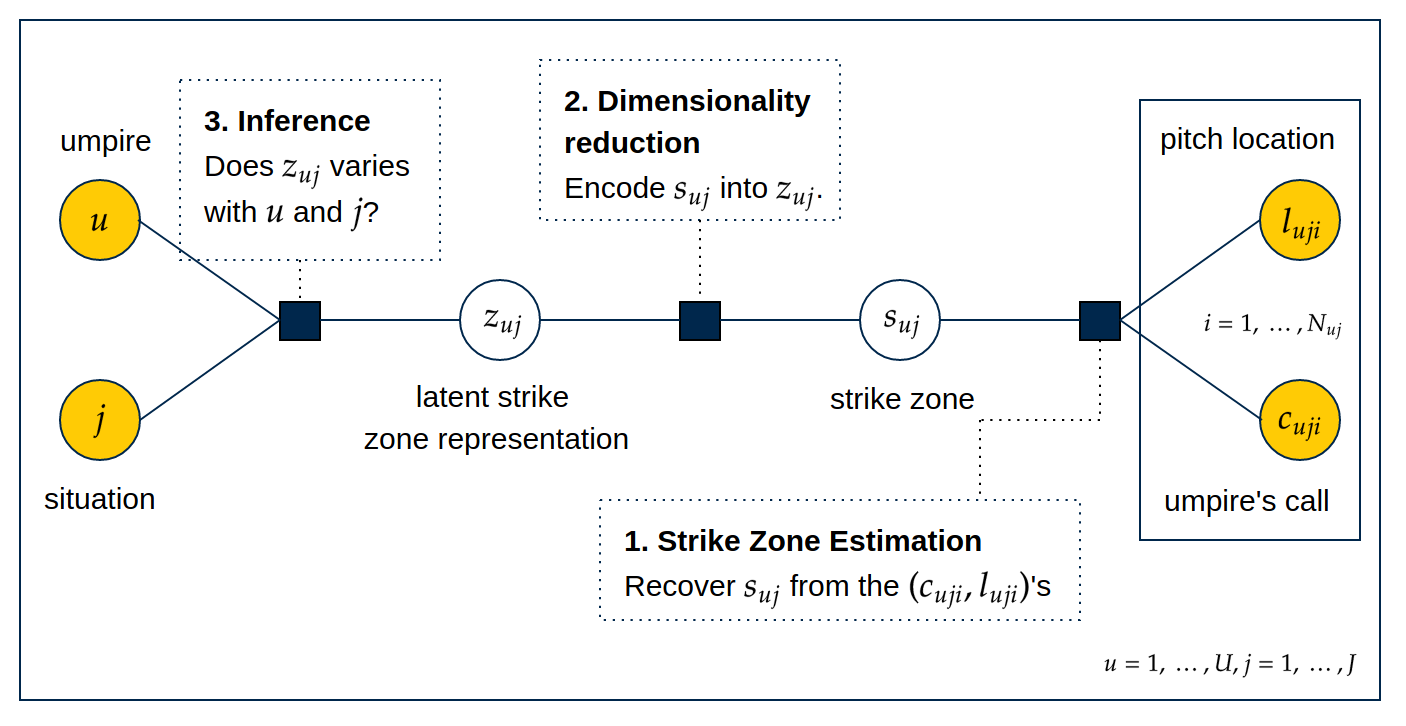
\includegraphics[scale=0.25]{fig/model_3.png}
    \caption{Graphical model for strike zone analysis}
    \label{fig:model_3}
\end{figure}

\begin{table}
\centering\small
\begin{tabular}{lp{8cm}rrrr}
\toprule
\multicolumn{3}{l}{\textbf{Experiments description}}& \multicolumn{3}{c}{Sample sizes}\\\cmidrule(l){4-6}
{} &                                                                                Splittings (levels) &  Count &  Min. &  Med. &  Max. \\
\midrule
1 &   Ball count ([0,2], {3}), Strike count ([0,1], {2}) &    156 &    96 &   470 &  4370 \\\addlinespace
2 & Horiz. movement (inward, outward), \newline Vert. movement (upward, downward) &    156 &   600 &  1032 &  2125 \\\addlinespace
3 & Pitcher's arm (L, R), Batter's stand (L, R) &    156 &   288 &  1336 &  2187 \\\addlinespace
4 & Batter's score diff. ($<$-1, [-1, +1], $>$+1), \newline Inning ([1,6], 7+) &    234 &   306 &   582 &  2401 \\
\bottomrule
\end{tabular}
\caption{Description of the experiments conducted. All splittings also include the 39 umpires.}
\label{tab:data.exps}
\end{table}


\Cref{fig:model_3} gives a graphical depiction of the problem we are exploring. 
We observe the pitch location and umpire's call, and use these two variables to learn the classifier (the strike zone).
We then need to reduce the dimension (using, e.g., PCA) of the strike zone to be able to perform inference at the next stage.
The inference portion of our model is where we explore whether the umpire and the situation, $u$ and $j$, have an effect on the size or location of the strike zone. 
The umpires are any of the 39 umpires in our sample and the situations are any combination of game outcomes mentioned in the previous paragraph (and listed in \cref{tab:data.exps}). 


%------------------------------------------------------------------------------
\subsection{Data Set}\label{sec:data}

MLB publishes the location of every pitch each season through its PITCHf/x data, which we retrieved for the 2018 season from Kaggle\cite{schale2019mlb}.
The PITCHf/x data includes the precise location of each pitch as it corsses the plate, the speed at which it travelled, its horizontal and verticle movements as it crosses the plate, as well as information about the game, such as the umpire and the players involved.
All that is needed to learn a classifier is the $x$ and $y$ coordinates of the pitches as well as the label--ball or strike--as called by the umpire.
We make use of the other ``covariates'' such as count, batter stance, or whether the pitcher is on the home team or away team, to judge umpires' consistency across game situations.

The data that we downloaded from Kaggle was relatively clean, but we did some minor preprocessing to facilitate our analysis.
The first step is to only consider the pitches that were not swung at, reducing our data set from 724,444 pitches to 364,099 pitches.
We next subset the data to only include umpires with at least 30 games as the home plate umpire during the 2018 season. 
This step was taken to ensure that the sample size for each umpire would be large enough for any game situation we consider, and also to ensure that we are only considering full-time professional umpires.
By restricting the data set to include games with experienced umpires, we were left with 182,558 pitches.
The next step was to clean the data by removing anything we believed to be an error in the data. 
An example of this would be a pitch with a negative $y$ coordinate, as the lowest possible $y$ coordinate is 0, which would indicate a ball that bounced before crossing home plate.
After cleaning the data, we are left with 178,922 pitches to consider in our analysis.

We also perform some standardization on the data set. 
Since the height of the strike zone changes based on the height of the batter, we standardize the strike zone for each player.
The data set includes two variables, \verb+sz_top+ and \verb+sz_bot+, which indicate the top and bottom of the strike zone, respectively, for the batter. 
We construct a linear map from these coordinates to the mean values of \verb+sz_top+ and \verb+sz_bot+ and then apply that map to the $y$ coordinate of the pitch, \verb+pz+, to get the standardized location for each pitch. 
The $x$ coordinate of the pitch, \verb+px+, specifies the distance from the center of home plate. 
Therefore, to make sure inside and outside pitches have the same sign for this variable regardless of a batter's stance, we switch the sign of \verb+px+ for left-handed batters.
Once these steps are complete, we are able to begin our analysis.

%------------------------------------------------------------------------------
\section{Classification}\label{sec:classification}
\begin{wrapfigure}{R}{0.33\textwidth}
\vspace{-0.6cm}
\centering
  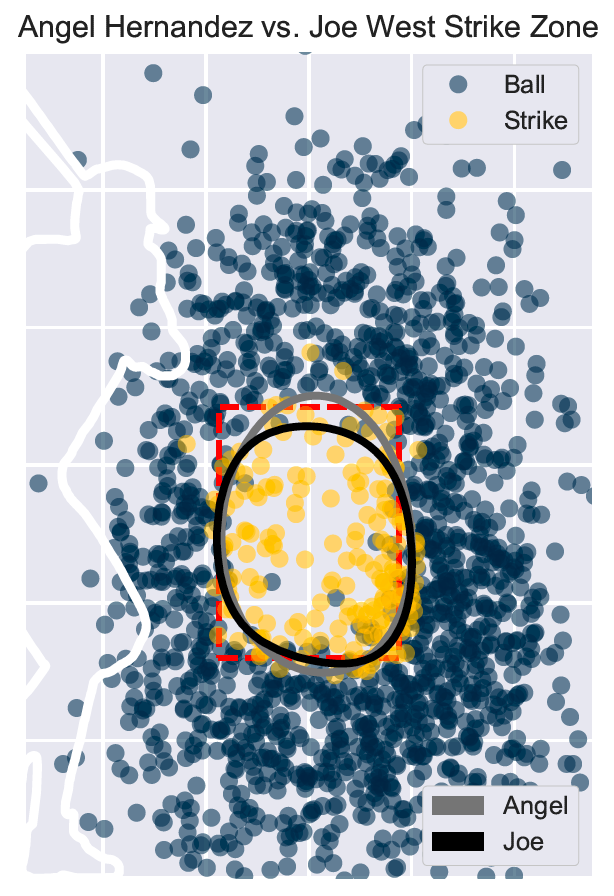
\includegraphics[scale=0.2]{graphics/batter.png}
  \caption{Example of two different strike zone classifiers}
  \label{fig:example-sz}
  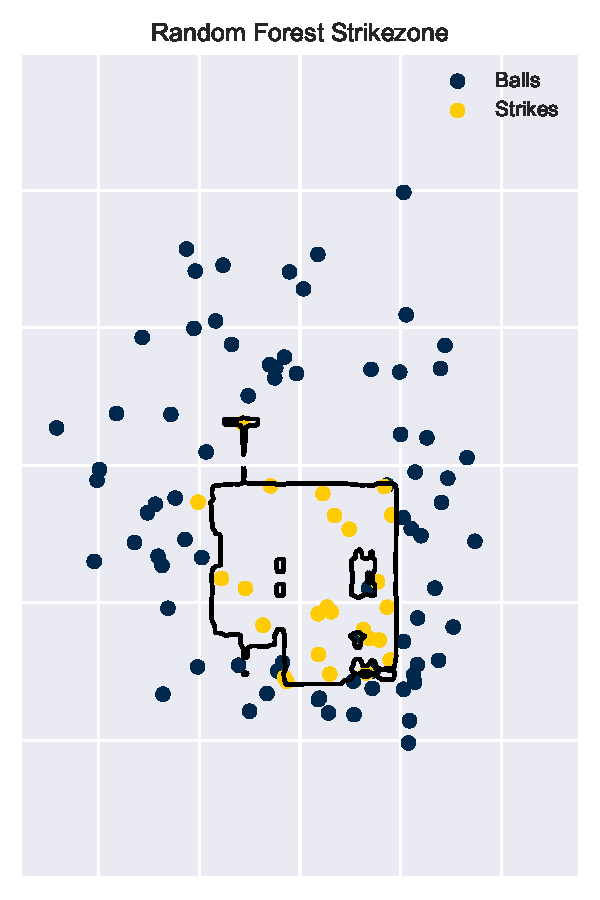
\includegraphics[scale=0.42]{graphics/RandomForeststrikezone.pdf}
  \caption{A random forest strike zone}
  \label{fig:rf-sz}
  \vspace{-0.64cm}
\end{wrapfigure}
Learning the strike zone for each umpire is a \textit{nonlinear} classification problem.
Given a two dimensional vector for each pitch (its $x$ and $y$ coordinate) and a label (the umpire's call of ball or strike), we want to learn the boundary that separates balls and strikes for each umpire (his strike zone).
In \cref{fig:example-sz} we see that there is a clear nonlinear boundary between balls and strikes, even if that boundary does not perfectly match the boundary specified in the rule book, which is indicated by the red dashed line.
The classifiers should (1) yield boundaries which both reflect the shape of the actual strike zone (meaning we shouldn't overfit to the few bad calls an umpire makes) and (2) minimize the cross validation error when comparing the actual labels called by the umpire to those predicted by our classifier.

We tried multiple methods to learn the umpires' strike zones for each unique game situation and we report the results of these methods on two different game situations in \cref{tab:classification.cv_results}.
As is expected for a low dimensional classification problem with a clear boundary, the cross validation error is low, even in the relatively small sample case where $n=150$.
%\moritz{Prefer to discuss performance more general level than one specific umpire. Would allow to include the sample size vs classification plot plus good overall results regardless of sample size, see italic}
For both scenarios, kernel logistic regression, kernel support vector machines, and a neural net yield the best CV scores. 
%\textit{\Cref{fig:class-cv-res} shows the classifiers' AUROC scores vs. sample sizes (excluding neural nets). While there is more variation in the quality of the classifiers for game situations with small sample sizes, large sample sizes do not produce uniformly better classifiers than small samples. This indicates that it is reasonable to compare strike zones even when sample sizes change.}
\Cref{fig:class-cv-res} shows the classifiers' AUROC scores vs. sample sizes (excluding neural nets). While there is more variation in the quality of the classifiers for game situations with small sample sizes, large sample sizes do not produce uniformly better classifiers than small samples. This indicates that it is reasonable to compare strike zones even when sample sizes change.
High AUROC is not enough to guarantee that our classifiers worked, however, as they also had to pass the visual test of actually looking like a strike zone (criterion 1 in the previous paragraph). 
As an example, \cref{fig:rf-sz} shows a strike zone fit by random forest, which does not resemble the shape of the real strike zone, even though it has a low classification error rate.
Therefore we decided to use KSVM and KLR for our classifiers in all cases (choosing the one between the two with a better AUROC) so that we would satisfy the criteria we established in the previous paragraph.

\begin{wrapfigure}[14]{R}{0.4\linewidth}
\centering
    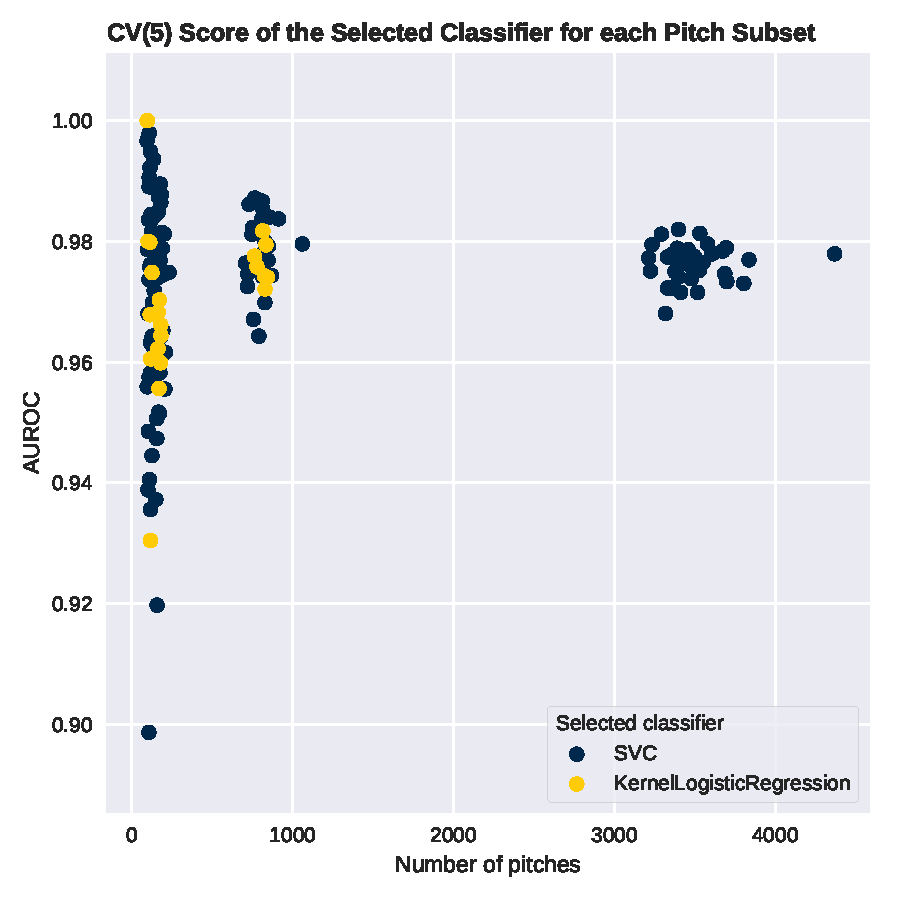
\includegraphics[scale=0.4]{graphics/classifiers_cv_results.pdf}
    \vspace{-0.7cm}
    \caption{CV results for KLR and SVC}
    \label{fig:class-cv-res}
\end{wrapfigure}

We are especially concerned about overfitting because of the inference procedures downstream from the classification. 
When we perform inference on the lower dimensional encodings of the strike zone, we need to be sure that the differences in encodings reflect the difference in the umpire's strike zones, and not the differences in classifiers. 
%\textit{Given the stark contrast of decision boundaries between KSVM and KLR classifiers versus tree-and ensemble base methods this is likely to happen if all methods are included. 
%Furthermore, due to the overfitting, even when only random forest classifiers are considered, dimension reduction techniques might pick up artifacts of overfitted strike zones rather than actual change in the judgment of the umpire.}
Given the stark contrast of decision boundaries between KSVM and KLR classifiers versus tree and ensemble based methods this is likely to happen if all methods are included. 
Furthermore, due to the overfitting, even when only random forest classifiers are considered, dimension reduction techniques might pick up artifacts of overfitted strike zones rather than actual change in the judgment of the umpire.
The random forest will be more sensitive to the precise location of the pitches, especially those with the ``wrong'' call, in the sample (thereby overfitting), whereas the SVC and KLR are more flexible and give shapes that are more consistent. 
This further supports our choice of classification methods in the analysis. 

\begin{table}
\centering\small
\begin{tabular}{lcccc}
\toprule
\multicolumn{1}{l}{\textbf{Classification results}}
 & \multicolumn{4}{c}{Score}\\\cmidrule(l){2-5}
Model &  AUROC &  Accuracy &  Balanced accuracy &  Brier \\
\midrule
\multicolumn{5}{c}{\textbf{3 balls ($n=150$)}}\\\addlinespace
AdaBoost 					&  0.900 &     0.847 &              0.841 & 0.173 \\
Gradient Boosting 			&  0.867 &     0.780 &              0.777 & 0.157 \\
Kernel Logistic Regression 	&  \underline{0.934} &     \underline{0.873} &              \underline{0.865} & \underline{0.106} \\
MLP 							&  \underline{0.934} &     \underline{0.880} &              \underline{0.872} & \underline{0.104} \\
Random Forest 				&  0.900 &     0.853 &              0.813 & 0.130 \\
SVC 							&  \underline{0.936} &     0.867 &              \underline{0.863} & \underline{0.108} \\
\midrule
\multicolumn{5}{c}{\textbf{{[0, 2]} balls ($n=3332$)}}\\\addlinespace
AdaBoost						&  {0.968} &     0.907 &              0.907 & 0.164 \\
Gradient Boosting 			&  {0.968} &     0.909 &              0.908 & 0.068 \\
Kernel Logistic Regression 	&  \underline{0.972} &     \underline{0.911} &              0.906 & \underline{0.065} \\
MLP 							&  \underline{0.972} &     \underline{0.913} &              0.908 & \underline{0.065} \\
Random Forest 				&  {0.967} &     0.909 &              0.908 & 0.069 \\
SVC 							&  \underline{0.972} &     0.908 &              \underline{0.910} & \underline{0.065} \\
\bottomrule
\end{tabular}
\vspace{1.5mm}
\caption{CV(5) scores for the selected model by four different criteria for two subsets (Joe West, {[0, 1]} strikes, {[0, 2]} or 3 balls).}
\label{tab:classification.cv_results}
\end{table}

%------------------------------------------------------------------------------
\section{Dimension Reduction}\label{sec:dimension}

Visual differences in strike zones may be obvious to baseball fans, but in order to attach statistical significance to these differences, we create low dimensional encodings of the strike zones.
The low dimensional encodings provide vectors on which we can do inference, using, e.g., multivariate regression. 
The first step in creating the encodings is to discretize the strike zone, evaluating the probability of a strike call at every point on a grid that spans the space of observable pitch locations. 
We then construct a data frame comprising the strike zone probability vectors for each combination of umpire and game situation and use principal components analysis and a convolutional neural net to create the low dimensional strike zone encodings.

To choose an appropriate dimensionality reduction method, we consider three criteria. 
irst, it has to produce an accurate representation of each strike zone as measured by the MSE between the reconstructed strike zones and the original strike zone. 
Second, we highly favor low-dimensionality in order to find a simple encoding as well as ease the future multivariate analysis. Third, we prefer methods producing \textit{orthogonal} embeddings since it produces more interpretable components and simplifies the incoming analysis. 
For example, this third criterion excludes \textit{(convolutional) neural network autoencoders}, which are an otherwise natural choice for image encoding---we can view the discretization of the strike zone as an image. 
While CNNs can achieve low MSE, the resulting embedding is much less interpretable due to its non-orthogonality. 
Hence, we identify that PCA and its kernel extensions both produce orthogonal components and thus we search for a simple and accurate encoder only within these two methods. 

\subsection{Principal Component Analysis}\label{sec:PCA}

\begin{wrapfigure}[11]{R}{0.5\linewidth} 
\centering
\vspace{-0.5cm}
  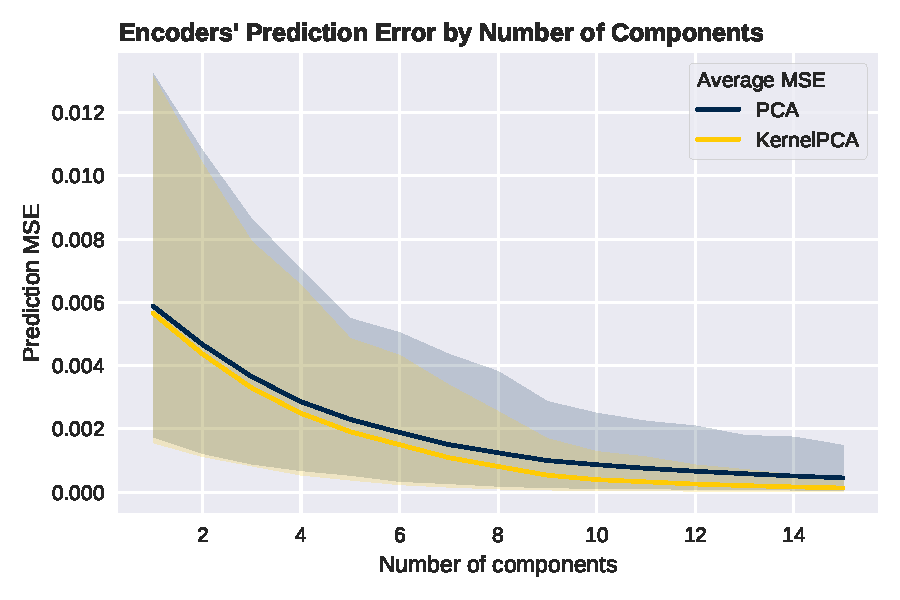
\includegraphics[scale=0.5]{fig/encoder_results.pdf}
  \vspace{-1cm}
  \caption{Prediction error by number of components}
  \label{fig:encoders}
\end{wrapfigure}
PCA yields orthogonal embeddings, which are desirable for inference, since fitting a multivariate regression to an orthogonal response vector is equivalent to separately fitting simple linear regression to each element of the vector.
We fit both PCA and Kernel PCA to the strike zone data. 
For Kernel PCA, we use a Gaussian kernel and perform cross-validation in order to select the scale and regularization parameters which minimizes the prediction MSE. 
\Cref{fig:encoders} shows the mean, min, and max prediction error by number of components for PCA and KPCA.
KPCA has a lower average MSE at every number of components, suggesting it will be a better encoding technique for our problem. 
Additionally, the max MSE for KPCA seems to level off at 10 components, so we used 10 components in our strike zone encodings when doing inference. 

\subsection{Components Interpretation}

In both cases, an advantage of the (K)PCA approach was that we were able to interpret the principal components by their orthogonal nature. 
Each component affects one part of the strike zone only through its own value.
Therefore, visual inspection of the effects of each component allows us to label them; these labels are of course arbitrary, but they still help in the interpretation of the results. 
The 10 components of the selected Kernel PCA model are labelled as follows, where their meaning is understood as the effect of a positive component value: the first component, \textit{Smaller}, shrinks the overall size; the second component, \textit{Uncertain}, produces a softer boundary; the third component, \textit{High inside excluded}, determines whether the upper left region is excluded; components four to six, \textit{Wide bottom, middle} and \textit{top}, expand the respective widths; the seventh component, \textit{NW/SE diagonal}, produces a diagonal shape; components eight to ten, \textit{Irregular 1, 2} and \textit{3}, yields irregular and less interpretable shapes. \Cref{fig:encoding.components} shows how the first five components affect the strike zone.

\begin{figure}
    \centering
    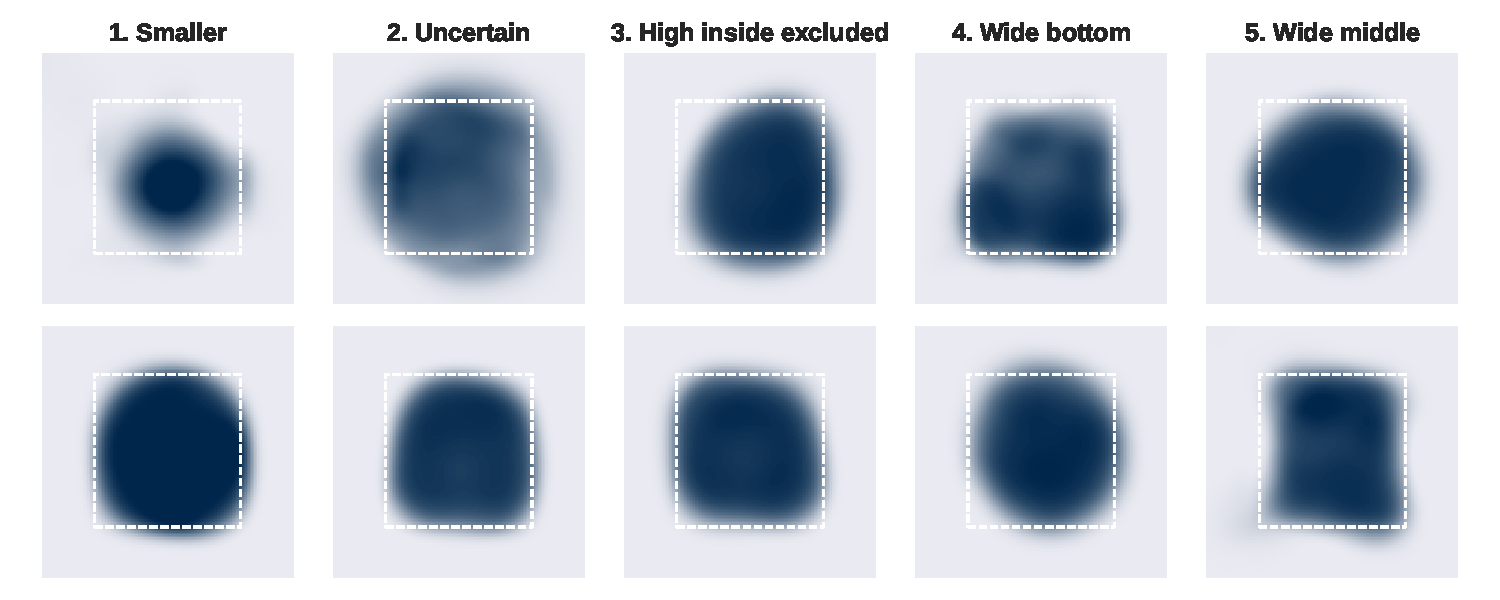
\includegraphics[width=\textwidth]{fig/encoding_components.pdf}
    \caption{Reconstructed strike zones by varying only one component from its maximal (top) to its minimal (bottom) observed value; other components are fixed to 0.}
    \label{fig:encoding.components}
\end{figure}

An important observation we find is that the second component is highly correlated with the sample size. This does not come as a surprise as smaller samples should produce less accurate classifiers and thus induce a less sharp boundary. We feel this is an interesting feature of the dimensionality reduction process as a single component is able to capture the sample size effect so that we can analyse the remaining components more confidently.

This interpretation of the principal components is useful because when we do inference later we will be able to determine not just \textit{if} certain factors are significant in changing the strike zone, but \textit{how} those factors affect the strike zone.

%------------------------------------------------------------------------------
\section{Inference}\label{sec:inference}

The third step in our analysis was to use different regression-based inference procedures to see which game situations affect the size and shape of umpires' strike zones. 
We consider four splittings: the count when the pitch is thrown, the horizontal and vertical movement of the ball as it crosses the plate, the handedness of the batter and pitcher, and the score and inning of the game when the pitch is thrown.
%The first method we use is to fit ANOVA on the principal components of the learned strike zones for each scenario separately. 
%We also fit a mixed effects multivariate regression model to the principal components where the umpire is a random effect, and we calculate the percent variance of the strike zone classifiers explained by the umpire random effect.
%With these two methods, we show how both the umpire and the game situation affect the strike zone the players see.

We proceed in two steps. First, to identify whether the features influence the overall strike zone, we conduct a \textit{multivariate analysis of variances} (MANOVA) in each experiment. 
Then, once we identify the effects that significantly influence the low-dimensional representation, we fit component-wise \textit{linear mixed models} (LMM) using the selected terms as fixed effects and umpires as random effects. 

\subsection{MANOVA}\label{sec:MANOVA}

For each experiment, we consider the multivaraite fixed effect model
\[
    \text{components}
    \sim
    \text{umpire} + \text{split 1}*\text{split 2}
\]
where $\text{components}$ is the 10-dimensional vector of components, $\text{umpire}$ is an intercept term for each umpire and $\text{split }i$ denotes one of the two additional features of the experiment. 
The model therefore consists of four relevant terms: the collection of umpire intercepts, the main effects of $\text{split 1}$ and $\text{split 2}$ and the interaction between $\text{split 1}$ and $\text{split 2}$. 
We identify terms that are significant at the 0.1\% level under Wilks' lambda test.

\Cref{tab:inference.manova} contains the results of the MANOVAs for the four experiments. In all four cases, the umpire intercept has a significant relationship with the vector of components. Our findings: only the main effects of ball count and strike count are important; the two-way interaction and the main effects of pitch movement and player handedness are significant; only the main effect of the inning influences the strike zone.


\begin{table}[t!]
\centering\small
\begin{tabular}{lrrrrr}
\toprule
\multicolumn{6}{l}{\textbf{MANOVA Results}}\\\addlinespace
                    Term & Wilks' lambda & Num DF &   Den DF &  F Value &  Pr $>$ F \\
\midrule
\multicolumn{6}{c}{\textbf{Ball and strike count}}\\\addlinespace
%               Intercept &        0.8074 &     10 &      105 &   2.5050 &  0.0097 \\
                  Umpire &        0.0142 &    380 &     1046 &   1.5181 &  0.0000 \\
              Ball count &        0.4112 &     10 &      105 &  15.0334 &  0.0000 \\
            Strike Count &        0.3553 &     10 &      105 &  19.0555 &  0.0000 \\
 Ball count:Strike count &        0.7675 &     10 &      105 &   3.1805 &  0.0013 \\
\midrule
\multicolumn{6}{c}{\textbf{Horizontal and vertical pitch movement}}\\\addlinespace
%               Intercept &        0.6391 &     10 &      105 &   5.9304 &  0.0000 \\
                  Umpire &        0.0022 &    380 &     1046 &   2.4258 &  0.0000 \\
              Horizontal &        0.4325 &     10 &      105 &  13.7767 &  0.0000 \\
                Vertical &        0.4624 &     10 &      105 &  12.2084 &  0.0000 \\
     Horizontal:Vertical &        0.5546 &     10 &      105 &   8.4335 &  0.0000 \\
\midrule
\multicolumn{6}{c}{\textbf{Pitcher's arm and batter's stand}}\\\addlinespace
%               Intercept &        0.7161 &     10 &      105 &   4.1629 &  0.0001 \\
                  Umpire &        0.0069 &    380 &     1046 &   1.8519 &  0.0000 \\
                 Pitcher &        0.3638 &     10 &      105 &  18.3618 &  0.0000 \\
                  Batter &        0.3205 &     10 &      105 &  22.2661 &  0.0000 \\
          Pitcher:Batter &        0.3827 &     10 &      105 &  16.9381 &  0.0000 \\
\midrule
\multicolumn{6}{c}{\textbf{Score and inning}}\\\addlinespace
%               Intercept &        0.9270 &     10 &      181 &   1.4253 &  0.1721 \\
                  Umpire &        0.0133 &    380 &  1782.16 &   2.6359 &  0.0000 \\
                   Score &        0.8282 &     20 &      362 &   1.7888 &  0.0204 \\
                  Inning &        0.7807 &     10 &      181 &   5.0838 &  0.0000 \\
            Score:Inning &        0.8139 &     20 &      362 &   1.9632 &  0.0084 \\
\bottomrule
\end{tabular}
\vspace{2mm}
\caption{Results from the multivariate analyses of variance on the components under four experiments.}
\label{tab:inference.manova}
\end{table}


\subsection{Component-wise Linear Mixed Models}\label{sec:LME}

For each experiment and each component, we consider a univariate linear mixed effect model
\[
    \text{component}
    \sim
    \text{umpire} + \text{selected terms},
\]
where now $\text{umpire}$ is treated as a random effect and $\text{selected terms}$ contains all terms selected from the MANOVA. The estimates from the fixed effects tell us about which component is affected by which feature as well as by how much and in which direction. 
\Cref{fig:ols_effects} contains a graphical representation of the estimated means of the significant univariate effects. 

First, a general appreciation of the results shows that the last three components of the encoding do not capture any difference in strikes zones. 
This result implies that we selected too many components at the dimensionality reduction step. 
Similarly, we do not find particularly strong effects beyond the first three components; we will thus only interpret the results for the \textit{Smaller}, \textit{Uncertain} and \textit{High inside excluded} components.

For the \textit{Smaller} component, we find that passing from a 2 strikes count to a fewer than 2 strikes decreases the component by \num{0.27}, indicating that umpires tend to substantially decrease the overall size of the strike zones when the count has 2 strikes. 
This result is not surprising as giving the third strike may have a large impact on the game and umpires may be reluctant to do so.
Also, we find a small difference between left-handed and right-handed batters in overall size and this effect seems to be well-known among the baseball analytics community \cite{lefty-zone}.

For the \textit{Uncertain} component, we remind the reader of the remark that it is strongly correlated with sample size.
Therefore, we refrain from commenting on the interpretation of these results as the effect of the features on the overall uncertainty is largely obfuscated by the rarity of the event and the corresponding performance of the classifier.

For the \textit{High inside excluded} component, we observe stronger effects for the handedness and pitch movement experiments. These two experiments are closely related because pitchers of a given handedness will almost always throw pitches with the same horizontal movement (right-handed pitchers generally have right-to-left movement and vice versa).
Now, corners of strike zones a very susceptible to pitch movement because the perceived location across the plate slightly changes with depth: this small change can be enough for an umpire to swing his call. 
Because we standardize horizontal pitch location for batter handedness, it is not surprising to see opposite effects when the batter's handedness is switched.

The variance estimate for the umpires' random effect can be used to study whether there is substantial variation between the baseline umpire strike zones when we account for the effects included in each model. 
For each experiment and each component, we compute the proportion of variance explained by the umpire's random effect (\cref{fig:lmm_pct_var}). This can be reinterpreted as a marginal $R^2$ statistic, which are typically used for the fixed effects, but can still inform us of the importance of the random effect.

\begin{figure}[t!]
    \centering
    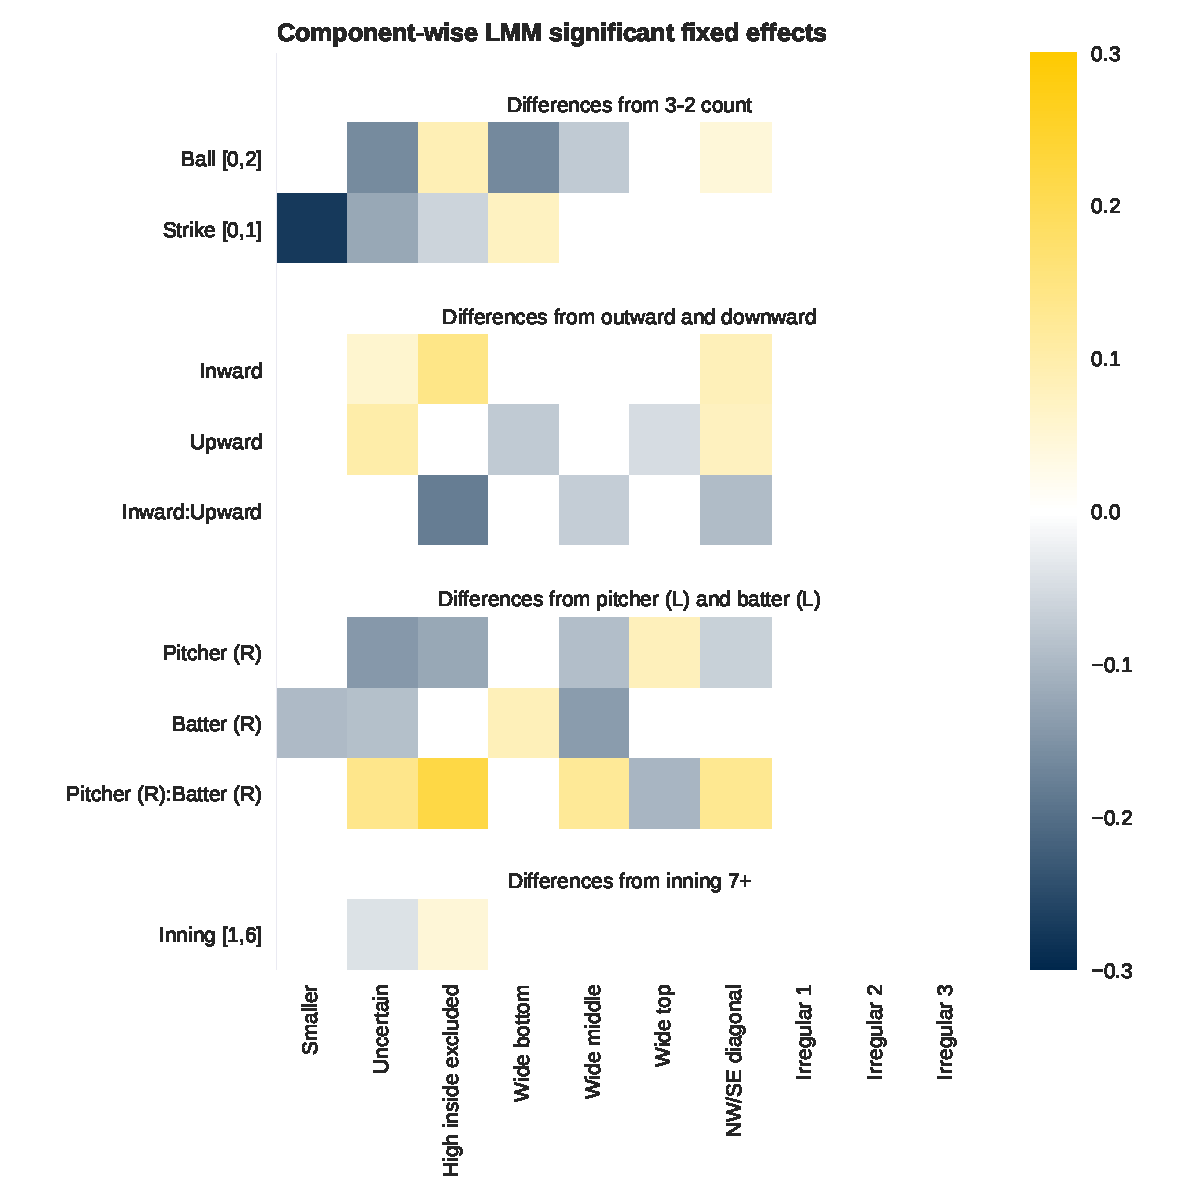
\includegraphics[scale=0.7]{fig/lmm_effects.pdf}
    \caption{Results from the component-wise linear mixed effect models applied to each experiment. Only effects significant at the 0.1\% level are shown.}
    \label{fig:ols_effects}
\end{figure}

We find that the variability across umpires manifests itself mostly through the overall size as well as through the widths components; there is much less variability beyond the first five components.
Conditional on the count, we observe that a small proportion of the variability is explained by the variability across umpires. 
When we do not account for that information (and account for some other), it seems umpires exhibit larger variability, especially with respect to overall size.
From this, we can understand that the count information captures a larger amount of variability than pitch movement, player handedness or game status.

\begin{figure}
    \centering
    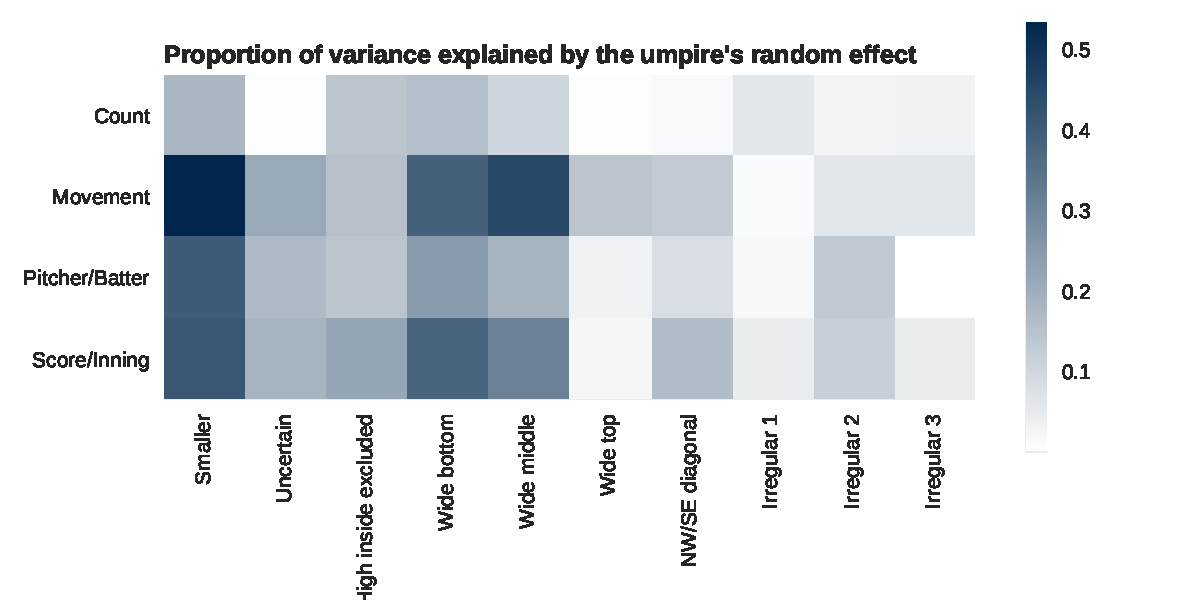
\includegraphics[scale=0.75]{fig/lmm_pct_var.pdf}
    \caption{Proportion of total variance explained by the umpires' random effect.}
    \label{fig:lmm_pct_var}
\end{figure}

%------------------------------------------------------------------------------
\section{Ranking Umpires}\label{sec:ranking}

\begin{wrapfigure}[14]{r}{0.45\linewidth} 
\centering
\vspace{-0.75cm}
  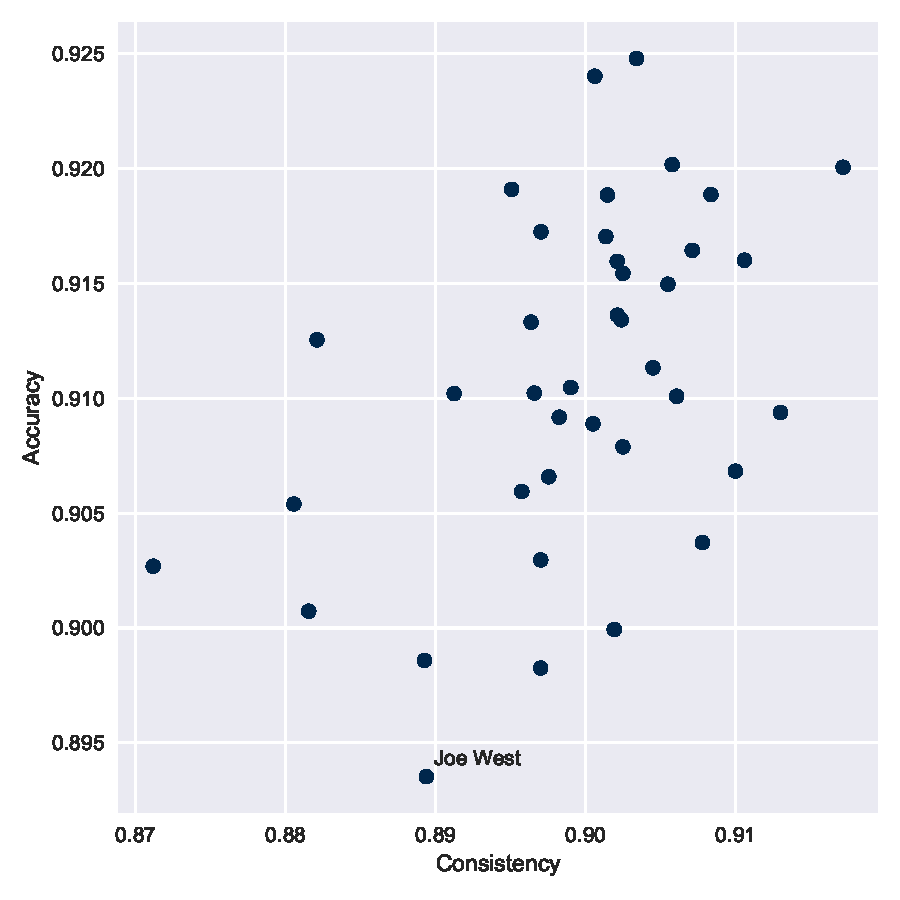
\includegraphics[scale=0.45]{graphics/Ranking.pdf}
  \vspace{-0.88cm}
  \caption{Comparison of accuracy and consistency}
  \label{fig:rankings}
\end{wrapfigure}

One way to get actionable insights from our analysis is through the construction of umpire rankings. 
Our procedure, unlike other ranking methodologies (cf. \cite{ump-audit} and \cite{bu-umps}), allows us to consider both the umpire's accuracy--the percentage of his calls that match the true strike zone, and his consistency--the extent to which his strike zone does not change across different game situations. 
We compute the umpire's accuracy score by comparing the call made by the umpire to the classification of the pitch according to the true strike zone and taking the percentage of correct calls. 
To compute the consistency score, we use a cross validation procedure. %\clearpage
For each umpire, we use each of his situation-specific strike zones and use it to classify all his pitches from the other situations. 
Then the misclassification error (according to the new labeling) is computed for each classifier and averaged to give the consistency score.

Our rankings weight accuracy 75\% and consistency 25\%. 
Accuracy is still more important than consistency, but players and coaches value knowing what to expect from umpires and having the ability to plan accordingly. 
\Cref{tab:ranks} compares our rankings to those compiled in \cite{ump-audit} and \cite{bu-umps}.
As an example of how our methodology influences the rankings, we look at Pat Hoberg, who appears second on the two external lists but is third on ours. 
Though Pat Hoberg had the second highest accuracy score in our sample (behind Mark Wegner), his consistency score was around the median, leading him to be surpassed by Vic Carapazza. 
Carapazza's consistency score was the highest in our sample, which led to him getting a boost in our rankings relative to those compiled by \cite{bu-umps}.
One can of course recompute our rankings with a different weighting scheme for accuracy and consistency (and see different results) but our main point is that consistency can be considered and stakeholders may find this beneficial.


\begin{table}
\centering\small
\begin{tabular}{lll}
\toprule
\multicolumn{3}{l}{\textbf{Umpire Rankings}}\\\addlinespace
                     This paper & Bloomberg \cite{ump-audit} &   Williams \cite{bu-umps} \\
\midrule
                          Mark Wegner &    Mark Wegner &  Mark Wegner  \\
                          Vic Carapazza &     Pat Hoberg &      Pat Hoberg \\
                        Pat Hoberg &     Alfonso Marquez &      Ryan Blakney  \\
                 John Tumpane &     Nic Lentz &      Vic Carapazza \\
                 Alfonso Marquez &     Sam Holbrook &      N/A\footnotemark \\
\bottomrule
\end{tabular}
\vspace{2mm}
\caption{Top 5 2018 umpires for umpires considered in our sample.}
\label{tab:ranks}
\end{table}
\footnotetext{Williams only publishes a top 10 for 2018, and only 4 of his top 10 are in our sample}

%------------------------------------------------------------------------------
\section{Discussion}\label{sec:discussion}

The authors of \cite{deshpande2017safe2} proceed to a very similar analysis as we are conducting. Indeed, they learn classifiers (GAMs) for each umpire and for each combination of batter and pitcher handedness. 
Then, they perform Bayesian logistic regression in order to study the effect of multiple covariates on the umpires' calls using the classifier as the fixed baseline. They are mostly interested in the question of ``framing'' pitches, but they also incorporate the count in their models. 
Our analysis is different in the sense that we train classifiers for each situation and compare these classifiers.

The sequential nature of our analysis introduces some possible pitfalls:
\begin{itemize}
    \item Since we need to train classifiers for subsets of data, this limits our analysis to the treatment of categorical features. For example, we needed to discretize counts, scores, innings and pitch movement into small numbers of bins. 
    \item Similarly, we need to ensure all subsets are relatively well-populated in order for the learned classifier to be minimally accurate. This limits the maximum number of subsets in each experiment; we found that beyond including the umpire effect it was not possible to include more than two discrete features.
    \item Additionally, we find that the sample size of each subset can potentially have a significant impact on the quality of the classifiers. Small sample sizes may lead to uncertain classifiers which was detected by the dimensionality reduction technique. We conjecture that the second component captured most of the variation due to sample size; the orthogonality of the components isolates this phenomenon which allows us to study the effect of the features where sample size is accounted for. Indeed, the relative rarity of some game situations should not impact our results.
    \item Related to the sample size is the pitch location sampling effect. Especially for smaller subsets, some regions of the 2-dimensional plane are occasionally less observed. The classifier trained on such subsets then have artificially higher uncertainty in regions where there should not be.
    \item Since only few features could be included in each experiments, multiple parallel experiments had to conducted to study the impact of all interesting features. This obviously leads to multiple testing issues: we tried to minimize this effect by choosing a fairly conservative significance level.
\end{itemize}
%- Since we need to train classifiers for subsets of data, this limits to the treatment of categorical features. For example, we needed to discretize counts, scores, innings and pitch movement into small numbers of bins. 
%- Similarly, we need to ensure all subsets are relatively well-populated in order for the learned classifier to be minimally accurate. This limits the maximum number of subsets in each experiment; we found that beyond including the umpire effect it was not possible to include more than two discrete features.
%- Additionally, we find that the sample size of each subset had a significant impact on the quality of the classifiers. Small sample sizes lead to uncertain classifier which was detected by the dimensionality reduction technique. We conjecture that the second component captured most of the variation due to sample size; the orthogonality of the components abstracts this phenomenon which allows us to study the effect of the features where sample size is accounted for. Indeed, the relative rarity of some game situation should not impact our results.
%- Related to the sample size is the pitch location sampling effect. Especially for smaller subsets, some regions of the 2-dimensional plane are occasionally less observed. The classifier trained on such subsets then have artificially higher uncertainty in regions where there should not be.
%- Since only few features could be included in each experiments, multiple parallel experiments had to conducted to study the impact of all interesting features. This obviously leads to multiple testing issues: we tried to minimize this effect by choosing a fairly conservative significance level.

Some possible fixes or possible improvements:

\begin{itemize}
    \item We have a very good idea of what strike zones look like and the variation between them should be minimal and contained in a small space (dimensionality reduction and inference found that fewer than 10 components was sufficient to roughly determine a strike zone). Using that information as part of the model could help alleviate two effects. First, it would diminish the sample size effect since we would have additional information coming from the prior knowledge. Second, the imperfect sampling of the space effect would be mitigated since the prior information would ``fill'' regions with fewer observations. There are many possible ways this could be achieved. A Bayesian approach could be used where the classifier (understood as a random function) would have a prior centered at an average strike zone. A parametric approach could also be used where only the regions on the boundary are allowed to change. The baseline approach suggested in \cite{deshpande2017safe2} could also be of interest here as we are interested in the deviations from a common strike zone. 
    \item Techniques from \textit{functional data analysis} could be used in the modeling of the strike zones directly as functions instead of using the discrete evaluations (e.g. \textit{functional PCA} \cite{shang2014survey}).
    \item A unified approach could potentially fix most of the problems induced by our sequential analysis. As depicted in \Cref{fig:model_3}, we consider a latent variable model, but we do not fit the model as a whole. Performing a single analysis on the complete model would allow the inclusion of all features in the same analysis as well as the use of continuous features. It would then fix the multiple testing issue and the two sampling issues as information would be shared more efficiently. Furthermore the observation that umpire's variability is lower when the count information is taken into account shows that a lot can be gained from a model that includes all features at once.
\end{itemize}
%- We have a very good idea of what strike zones look like and the variation between them should be minimal and contained in a small space (dimensionality reduction and inference found that fewer than 10 components was sufficient to roughly determine a strike zone). Using that information as part of the model could help alleviate two effects. First, it would diminish the sample size effect since we would have additional information coming from the prior knowledge. Second, the imperfect sampling of the space effect would be mitigated since the prior information would ``fill'' regions with fewer observations. There are many possible ways this could be achieved. A Bayesian approach could be used where the classifier (understood as a random function) would have a prior centered at an average strike zone. A parametric approach could also be used where only the regions on the boundary are allowed to change. The baseline approach suggested in \cite{deshpande2017safe2} could also be of interest here as we are interested in the deviations from a common strike zone. 
%- Techniques from \textit{functional data analysis} could be used in the modeling of the strike zones considered directly as functions instead of using the discrete evaluations (e.g. \textit{functional PCA} \cite{shang2014survey}).
%- A unified approach could potentially fix most of the problems induced by our sequential analysis. As depicted in \Cref{fig:model_3}, we consider a latent variable model, but we do not fit the model as a whole. Performing a single analysis on the complete model would allow the inclusion of all features in the same analysis as well as the use of continuous features. It would then fix the multiple testing issue and the two sampling issues as information would be shared more efficiently. Furthermore the observation that umpire's variability is lower when the count information is taken into account shows that a lot can be gained from a model that includes all features at once.



%------------------------------------------------------------------------------
\section{Conclusion}\label{sec:conclusion}
Our project seeks to answer the broad question of what factors affect the size and shape of the strike zone that professional baseball players see in each game. 
We begin by using nonlinear classification methods including kearnel logistic regression and support vector machines to create probabilistic representations of each umpire's strike zone.
Next we use kernel PCA to create low dimensional encodings of the strike zones learned in the first step.
We then do inference, including ANOVA and linear mixed effects models to determine what factors are most significant in determining the size and shape of the strike zone.
Finally, we use our methodology to come up with a composite ranking score for the umpires in our sample that combines their overall accuracy (with respect to the true strike zone) and their consistency across game situations.

One area which we do not consider is the impact of the umpires' inconsistency on game outcomes. 
Further work could explore the number of games which may have had a different outcome if the umpire's accuracy or consistency was improved. 
By focusing on pitches that were misclassified by the standards of the rule book, analysts could incorporate other research in Sabermetrics to quantify the number of runs an umpire created or took away through his missed calls.

Ultimately, the question of whether MLB should incorporate more technology when officiating its games is one only the league can answer. 
The overthrowing of over 100 years of tradition should not be taken lightly.
With billions of dollars on the line (and the prise of winning--which cannot be valued with money), however, teams and their players should be able to expect the fairest possible treatment from game officials. 
We hope that our contribution can help move the debate forward to ensure a long and successful future for the sport of baseball. 


%% BibTeX support
\bibliographystyle{DeGruyter}
\bibliography{utils/strikezone}

\end{document}